\chapter{Technische Grundlagen} \label{Technische_Grundlagen}

\section{Internet Protocol Version 4 (IPv4)} \label{ipv4}
\subsection{Allgemeines und Adressierungsschema}
Das Internet Protocol ist im OSI-Modell auf Schicht 3 (Network-Layer) anzusiedeln. Es dient der \textit{Paketierung} von Daten und anschließenden Ende-zu-Ende-Vermittlung dieser \textit{Pakete} zwischen Netzwerk-Systemen. Dafür notwendig ist eine Adressierung: eine IPv4-Adresse besteht aus einer 32 Bit-Zahl, welche typischerweise dezimal dargestellt wird in so genannter \glqq dotted decimal\grqq{}-Schreibweise. Dafür wird die Binärzahl in vier Oktette mit einem Punkt aufgeteilt und die jeweiligen Oktette in dezimal umgerechnet.

00000001000000100000001100000100 (32-Bit Integer) ->  00000001.00000010.00000011.00000100 (dotted binary) -> 1.2.3.4 (dotted decimal)

Mit Hilfe von Netzmasken wird die Netzwerkgröße bestimmt. Der Host mit der IP-Adresse 1.2.3.4 und einer Netzmaske von bspw. 255.255.255.0. Diese Netzmaske entspricht in dotted binary:

11111111.11111111.11111111.00000000

Die ersten 24 Bit sind für das Netzwerk reserviert (Network bits), die letzte 8 Bit sind Host bits. Dieses Netzwerk kann somit theoretisch aus $2^8 = 256$ Hosts bestehen, wobei die erste und letzte Adresse reserviert sind (Netzwerkadresse und Broadcast-Adresse).

Heutzutage üblich ist die so genannte CIDR-Notation, welche IP-Addresse und Subnetzmaske vereint. Wenn man die erwähnten Beispiele aus Adresse und Subnetzmaske zusammenführt, erhält man die IP-Adresse in CIDR-Notation: 1.2.3.4/24. /24 entspricht dabei den gesetzten Network bits.

Mit Hilfe der IP-Adresse und Netzmaske lässt sich ermitteln, ob sich ein anderer Host im gleichen \textit{Subnetz} befindet. Dafür berechnet man die Netzwerkadresse per logisch-AND:

\begin{lstlisting}[label=local-ip-address-AND-subnet,caption=Blub]
... 00000001.00000010.00000011.00000100
AND 11111111.11111111.11111111.00000000
  = 00000001.00000010.00000011.00000000 => Netzwerkadresse: 1.2.3.0/24
\end{lstlisting}
    
Hat man nun zwei Hosts 1.2.3.240 und 8.9.10.23, mit denen man eine IP-Verbindung aufbauen will, so prüft der Initiator zuerst, ob das jeweilige Netz \textit{link-lokal} erreichbar ist, also im gleichen IP-Netzwerk wie der Initiator liegt.

Für 1.2.3.240:

\begin{lstlisting}[label=local-ip-address-AND-subnet-same,caption=Blun]
... 00000001.00000010.00000011.11110000
AND 11111111.11111111.11111111.00000000
  = 00000001.00000010.00000011.00000000 => Netzwerkadresse: 1.2.3.0/24 (gleiche Netzwerkadresse wie oben, link-lokal erreichbar)
\end{lstlisting}

Für 8.9.10.23:

\begin{lstlisting}[label=local-ip-address-AND-subnet-different,caption=Blub]
... 00001000.00001001.00001010.00010111
AND 11111111.11111111.11111111.00000000
  = 00001000.00001001.00001010.00010111 => Netzwerkadresse: 8.9.10.0/24 (andere Netzwerkadresse: das Paket muss \textit{geroutet} werden)
\end{lstlisting}

\subsection{RFC 1918-Adressen}
%https://datatracker.ietf.org/doc/html/rfc1918
Ein Großteil der IP-Adressen werden \textit{blockweise} an Provider, Firmen und Forschungseinrichtungen herausgegeben und können fortan im Internet genutzt werden. Mit RFC 1918  wurden Blöcke durch die IANA reserviert, welche ausschließliche für private und firmeninterne Nutzung vorgesehen sind. Sie werden im Internet nicht geroutet. Es handelt sich dabei um die Blöcke:
\begin{itemize}
\item 10.0.0.0/8
\item 172.16.0.0/12
\item 192.168.0.0/16
\end{itemize}

Auf diese Blöcke wird auch in der Bachelor-Arbeit zurückgegriffen, um Zugriff auf \textit{interne}, vom Internet \textit{isolierte} Ressourcen zu ermöglichen.

\subsection{IP-Routing}

Wie im vorherigen Beispiel gefolgert, müssen Pakete, die Ziele in anderen Subnetzen haben, geroutet werden. Dafür besitzen alle Netzwerkteilnehmer eine Routing-Tabelle, um herauszufinden, an welchen \glqq Next-Hop\grqq{} ein Paket adressiert werden muss. Im folgenden Beispiel besteht das Netzwerk aus vier Teilnehmern: einem Client, einem Server und zwei Routern (R1 und R2). Alle Geräte verwalten eine Routing-Tabelle, in denen die Zielnetze und Next-Hops vermerkt sind.
Damit weiß der Client, dass Pakete für das Netzwerk 192.168.200.0/24 über R1 mit der IP-Adresse 192.168.0.1 geschickt werden müssen. R1 nimmt das Paket an, schaut wiederum in der eigenen Routing-Tabelle nach und schickt das Paket dann weiter an R2, usw. (Rück-)Pakete vom Server zum Client durchlaufen die gleiche Prozedur pro Hop.\\
Client und Server müssen im Übrigen das Netzwerk 192.168.100.0/30 \textbf{nicht} in ihrer Routing-Tabelle pflegen. Dieses Netzwerk hat ausschließlich eine Relevanz zur Übertragung von Daten zwischen R1 und R2: Man spricht auch von Transfernetzwerken.\\

\begin{figure}[h]
  \centering
  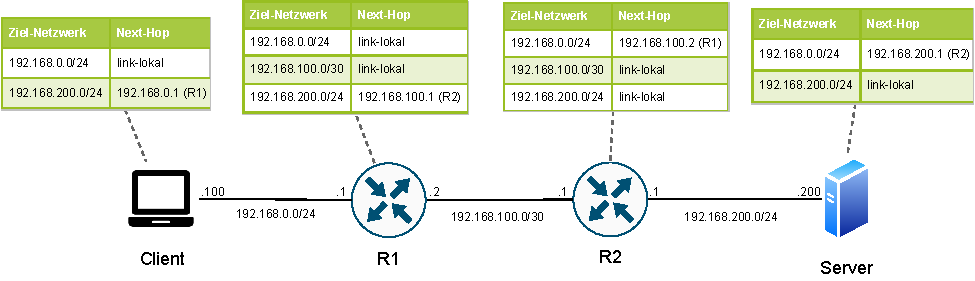
\includegraphics{Figures/next_hop_routing_specific_table.pdf}
  \caption{Next Hop Routing}
  \label{grafik: next_hop_routing}
\end{figure}

Dieses Beispiel bringt ein Skalierungsproblem mit sich: Umso mehr Subnetze existieren, in denen Server zu erreichen sind, desto mehr Routen muss der Client in der Routing-Tabelle, u.U. manuell gepflegt, vorhalten. Das gleiche gilt für Server, insofern eine Server-zu-Server-Kommunikation gewünscht ist.\\
In der Praxis sieht man kaum noch Endsysteme (darunter fallen Client und Server), welche mit solchen \textit{spezifischen} Routen arbeiten. Man überlässt die komplexe Verwaltung von Routing-Tabellen den Routern, während die Endsysteme neben der link-lokalen nur noch die \textit{Default}-Route besitzen. In diese Route 0.0.0.0/0 fallen alle Zielnetzwerke, abgesehen vom link-lokalen Subnetz, und sie zeigt immer auf den lokal erreichbaren Router.\\
Das Setzen der Default Route garantiert allerdings nicht, dass ein Ziel auch wirklich erreicht werden kann, z.B. weil es gar nicht existiert oder das Zielnetzwerk nicht in der Routing-Tabelle eines (Next-Hop-)Routers vorhanden ist. Ein Hilfsprotokoll zur Signalisierung von Erreichbarkeit ist dabei das Internet Control Message Protocol (ICMP). Das bekannte Werkzeug \textit{ping} nutzt Nachrichten in Form von ICMP Echo Request und ICMP Echo Response, um die Erreichbarkeit via IP eines Endsystems zu prüfen.
\begin{figure}[h]
  \centering
  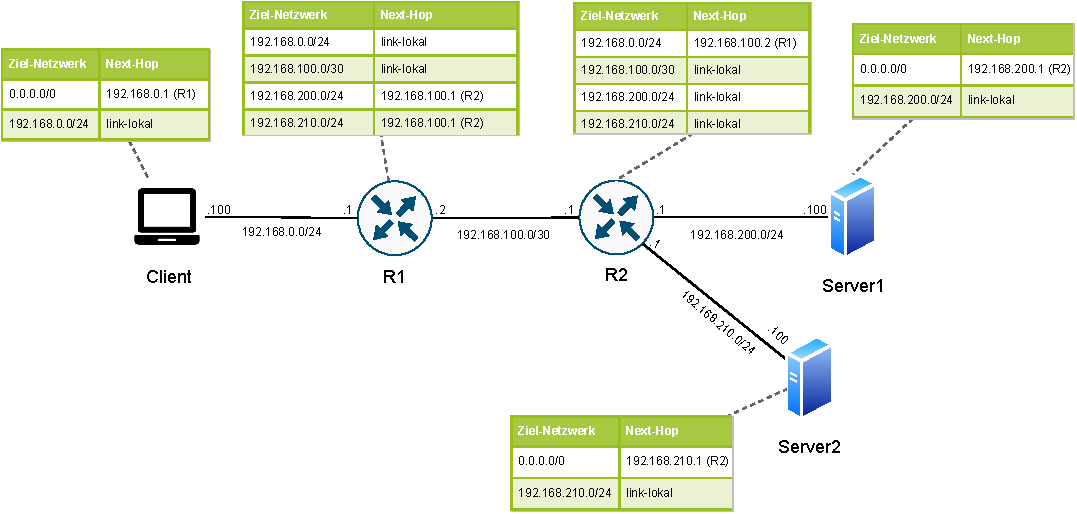
\includegraphics{Figures/next_hop_routing_default_route.pdf}
  \caption{Next Hop Routing mit Default Route}
  \label{grafik: next_hop_routing_with_default_route}
\end{figure}\FloatBarrier

Prinzipiell spielen im IPv4-Routing viele weitere Mechanismen eine zentrale Rolle: Zu nennen wären an dieser Stelle bspw. MAC-Adressen (Ethernet), Address Resolution Protocol (ARP), administrative Distanz und Time-To-Live (TTL). Für diese Ausarbeitung haben die Themen allerdings keine Relevanz. Das Thema \glqq dynamisches Routing\grqq{} wird später noch behandelt.

\textbf{\underline{Statisches IP-Routing}}\\
Wenn man das vorherige Listing (...) noch einmal betrachtet, dann gibt es zwei Next-Hop Typen: link-lokal und \glqq IP-Adresse\grqq{}. Die link-lokale Route wird automatisch angelegt, sobald eine Netzwerk-Schnittstelle mit den entsprechenden Adressparametern konfiguriert wird.\\
Routen hingegen, die als Next-Hop eine IP-Adresse beinhalten, müssen entweder als statische oder dynamische Route den Weg in die Routing-Tabelle finden. Statische Routen sind Routen, bei denen ein Administrator Ziel-Netzwerk und Next-Hop manuell auf den Geräten pflegt. Käme in Beispiel (Listing...) ein drittes Netzwerk \glqq Server3\grqq{} hinzu, müsste auf Router R1 eine statische Route zu diesem Ziel mit dem Next-Hop 192.168.100.1 eingetragen werden, damit IP-Pakete von Client das Server3-Netzwerk erreichen.\\
Bis zu einer gewissen Netzwerkgröße lassen sich die Routing-Einträge statisch pflegen. Ab größeren Skalierungen mit vielen Routern wird die Administration jedoch problematisch. So kann es passieren, dass Router in der Konfiguration vergessen werden und lokale Routing-Einträge fehlen: dies macht eine Weiterleitung dann unmöglich und die Pakete werden verworfen.\\
Weiterhin bieten statische Routen wenig Flexibilität, wenn Verbindungen ausfallen. Es ist zwar möglich, Backup-Routen zu definieren, die zum gleichen Ziel über einen anderen Next-Hop führen. Dafür würde man diese Routen mit einer schlechtern \textit{Metrik} versehen. Allerdings ist es ab einer gewissen Anzahl von Routern unmöglich, alle \textit{Fallback-Szenarien} vorab zu durchdenken.
%Routing Bild mit Dreieck

\textbf{\underline{Dynamisches IP-Routing}}\\
Dynamische Routing-Protokolle können die genannten Probleme (s.o.) umgehen, indem sie manuelle Administrationsaufwände verringern bzw. verhindern. Router, die ein dynamisches Routing-Protokoll nutzen, können gegenüber benachbarten Routern Erreichbarkeit für bestimmte Netzwerke signalisieren. Diese Information wird dann über die immer weitere Nachbarn weitergetragen und so erhalten alle berechtigten Router einer \textit{Routing-Domäne} die Information, \textit{welche} Netzwerke erreichbar sind und \textit{wie} sie erreicht werden können. Auch Fallbacken-Szenarien sind durch dynamische Routing-Protokolle abgedeckt. Meist werden Backup-Routen schon im Speicher vorgehalten, um bei Ausfall einer Leitung das Routing zu \textit{schwenken}.

\textbf{\underline{Border Gateway Protocol v4 (BGP)}}\\
Im Folgenden soll das Routing-Protokoll BGP betrachet werden. Dieses ist durch die Public Cloud-Provider vorgegeben, wenn dynamisches Routing gewünscht ist. Es ist ein so genannten AS-Pfadvektorprotokoll. AS steht dabei für Autonomous System: Ein AS kann als eine administrative \glqq Grenze\grqq{} für eine Gruppe von Routern aufgefasst werden. Tauschen Router per BGP Routing-Informationen aus, spricht man auch von einem \textit{BGP-Peering}. Man unterscheidet an dieser Stelle zwischen internal BGP (iBGP) und external BGP (eBGP): Peerings innerhalb eines AS sind iBGP-Peerings, Peerings über AS-Grenzen hinweg sind eBGP-Peerings. iBGP dient vor allem dem Zweck, per eBGP gelernte Routen (fortan \textit{BGP-Präfixe} genannt) innerhalb eines AS weiterzutragen.

\begin{figure}[h]
  \centering
  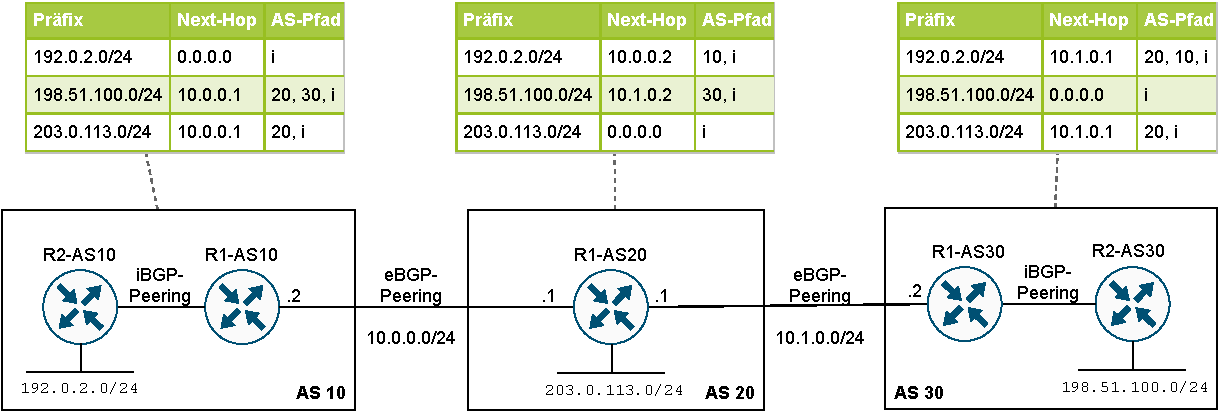
\includegraphics{Figures/ebgp_peerings.pdf}
  \caption{Beispielbild eBGP / iBGP Speaker}
  \label{grafik: ebgp_peerings}
\end{figure}\FloatBarrier

Wie man auf dem Bild sieht, werden drei Präfixe aus drei verschiedenen AS bekannt gemacht. Der AS-Pfad zeigt an, über welche AS ein Präfix erreicht werden kann. \texit{i} steht dabei für internal und stellt immer den Ursprung des Präfixes dar: der Pfad wird von rechts (Ursprung) nach links (letztes AS vor dem eigenen - \glqq Nachbar\grqq).\cite{odom2010}

Anmerkung: R2-AS10 kann mit dem Next-Hop 10.0.0.1 aus der Tabelle nichts anfangen: Dieser ist nur für R1-AS10 erreichbar. Im iBGP nutzt man daher das Attribut Next-Hop-Self, womit iBGP-Nachbarn signalisiert wird, dass Next-Hop-Erreichbarkeit für ein Präfix \textit{über einen selbst} gegeben ist.\cite[S.468-471]

\begin{figure}[h]
  \centering
  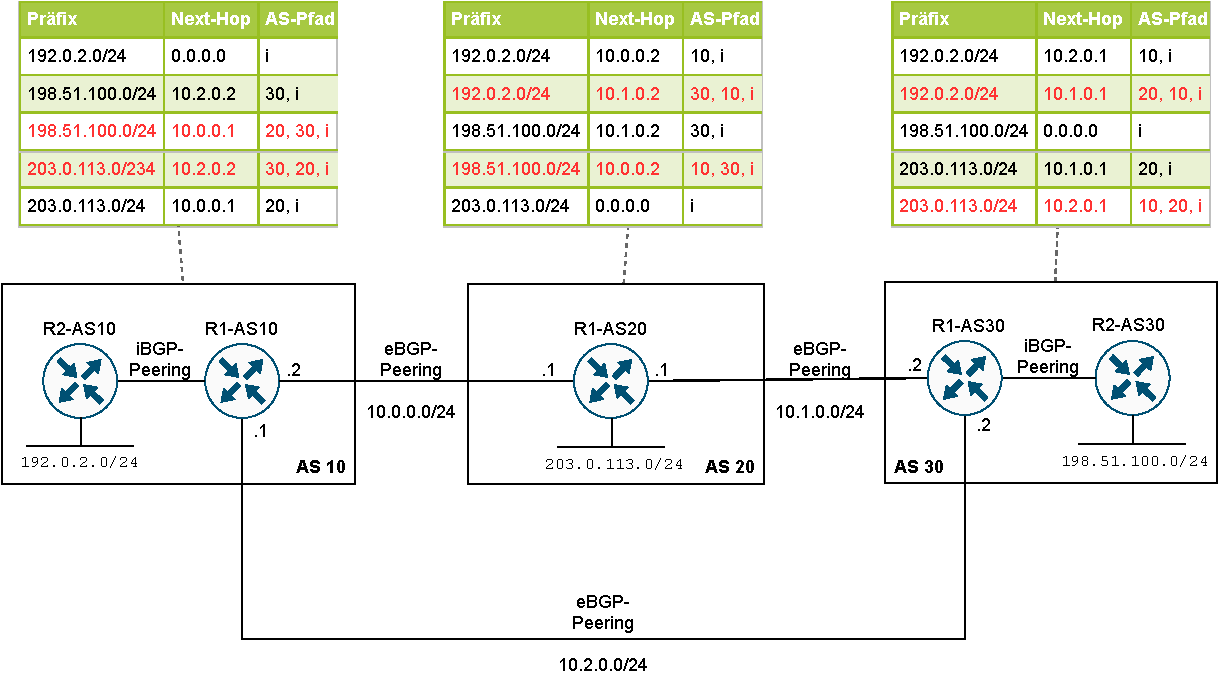
\includegraphics{Figures/ebgp_peerings_additional_connection.pdf}
  \caption{Beispielbild eBGP / iBGP Speaker mit weiterer Verbindung}
  \label{grafik: ebgp_peerings_additional_connection}
\end{figure}\FloatBarrier

In diesem Beispiel wurde noch eine Verbindung zwischen AS 10 und AS 30 hinzugefügt. Damit werden alle Präfixe, bis auf die eigenen, doppelt sichtbar, da sie nun über verschiedene Pfade erreicht werden können. Im Standardfall wird das Präfix mit dem kürzeren AS-Pfad bevorzugt. Die Präfixe mit roter Schriftart sind dabei allerdings nicht nutzlos. Sie können als Backup-Pfad dienen, falls der bessere Pfad wegfallen sollte. Falls bspw. die Verbindung zwischen AS 10 und AS 30 ausfällt, \textit{konvergiert} das BGP auf allen Routern wieder hin zu Fall 1 (Listing...).

https://datatracker.ietf.org/doc/html/rfc4271#section-9.1.2
BGP-Router ignorieren AS-Pfade, in denen die eigene AS-Nummer bereits vorkommt. Pakete werden dann gemäß RFC verworfen werden. Dadurch werden effektiv Routing-Schleifen verhindert.

%https://datatracker.ietf.org/doc/html/rfc6996
BGP sieht analog zu RFC 1918-Adressen Bereiche für AS-Nummern vor, die privat, also nicht im Internet, verwendet werden dürfen. Diese gehen von einschließlich 54512 bis 65534.

%Cisco Doku
%next-hop self?
%BGP hat noch weitere \textit{Tie-Breaker}...
%AS-Pfad dient auch der Schleifenverhinderung
%64512–65534
%Beispieldiagramm


%Typische IGPs sind: OSPF, EIGRP, RIP, IS-IS
%Heutzutage findet nur noch ein EGP Verwendung: BGP

%Transfernetzwerk
%keine Metrik / AD
%Next Hops in Cloud funktionieren anders...
%In den Ursprüngen des Internets waren IP-Adressen \textit{classful}: die Netzwerkgröße wurde über die Klassenzugehörigkeit einer IP-Adresse bestimmt. Ein Class A Netz fiel in die \textit{Range} 0.0.0.0 - 127.255.255.255. So hätte obige IP-Adresse zu dem Class-A-Netzwerk "1.0.0.0" gehört

\subsection{Network Address Translation (NAT)}
%https://countrymeters.info/de/World
Grundlegend geht es bei NAT darum, eine IP-Adresse \textit{umzuschreiben}. Dies ist sowohl für die Absender- als auch die Ziel-Adresse möglich. Dies kann verschiedene Gründe haben, die meisten NAT-Mechanismen beruhen aber auf der grundlegenden Idee, IPv4-Adressen einzusparen. Dies ist dem Umstand geschuldet, dass IPv4 nur einen Adressraum von 32 Bit hat, was $2^{32} \approx 4.000.000.000$ Adressen entspricht. Wenn man dagegen hält, dass die Weltbevölkerung bereits knapp $8.000.000.000$ Menschen beträgt und viele Menschen bereits mehr als ein Endgerät besitzen, reicht der Adressraum bei weitem nicht mehr aus.\\
Langfristig soll IPv6 mit einem Adressraum aus $2^{128}$ Bit IPv4 ablösen, doch selbst im Jahr 2021 fehlt weiterhin die \textbf{vollständige Unterstützung} einiger Hersteller für IPv6. Dies gilt auch für die Public Cloud-Plattformen.\\
Der häufigste NAT-Mechanismus ist Network Address Port Translation (NAPT). Dabei können $n$ Clients hinter einer einzigen IPv4-Adresse \glqq verborgen\grqq{} und so IP-Adressen eingespart werden. Dafür werden neben der IP-Adresse bspw. noch Information der Transport-Schicht (Layer 4) wie Ports herangezogen, um NAPT-Sessions zuordnen zu können. Ein Router verwaltet diese Sessions in Form einer NAPT-Tabelle. Diese wird notwendig, wenn Rückpakete die verborgenen Clients erreichen sollen.
In dieser Ausarbeitung ist, wenn von NAT oder NATting gesprochen wird und keine anderweitigen Aussagen getroffen werden, der NAPT-Mechanismus gemeint.\\
Im Beispiel werden drei Clients hinter einem Router geNATtet. Alle eingehenden Pakete werden auf die Quell-IP 10.1.0.1 umgeschrieben und es wird ein neuer Quell-Port vergeben. Wenn nun eine Verbindung von einem Client initiiert wird, sieht der Webserver lediglich die Quell-IP und den Quell-Port des Routers, welche durch das NAT vergeben wurden. Rückpakete vom Webserver zu einem Client werden folgerichtig an den Router adressiert, welcher wiederum in der NAT-Tabelle nachschaut und die Pakete an den Client weiterleitet. Dafür müssen die Pakete auf das ursprüngliche Tupel aus Quell-IP und Quell-Port umgeschrieben werden.\\

\begin{figure}[h]
  \centering
  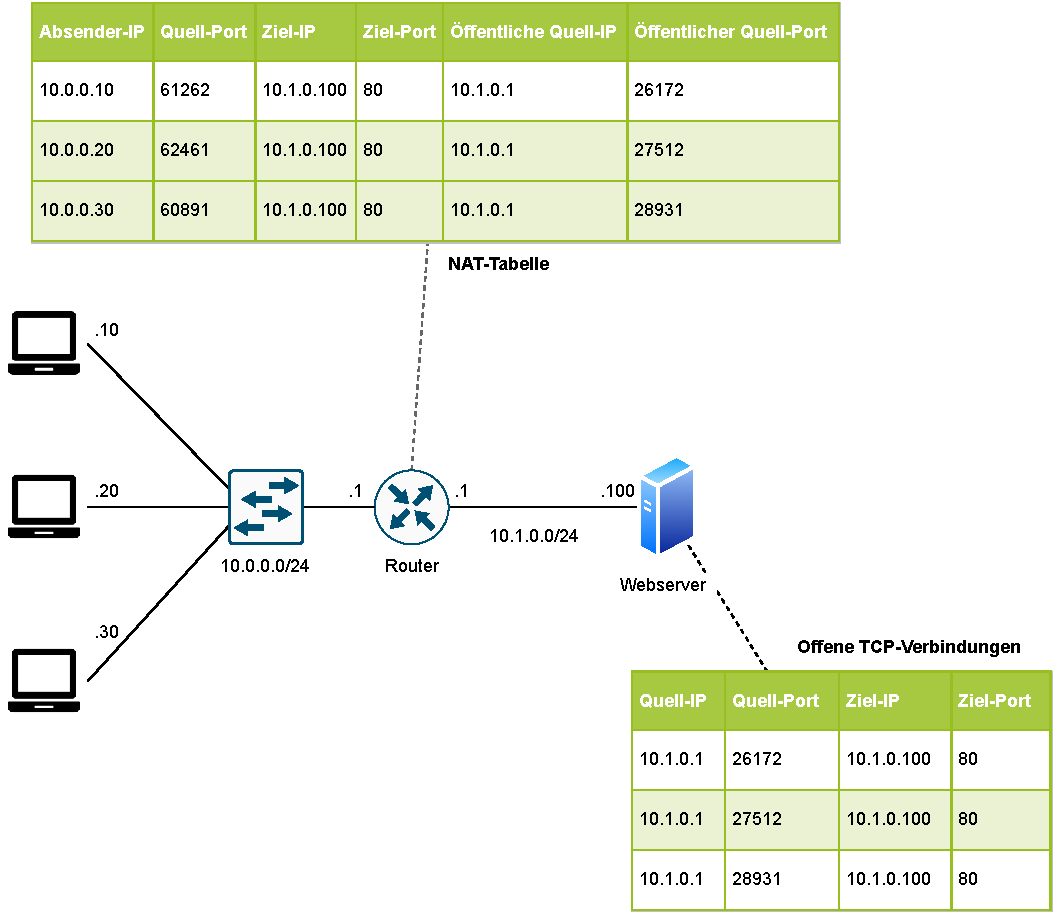
\includegraphics{Figures/napt.pdf}
  \caption{Beispiel Network Address Translation}
  \label{grafik: napt}
\end{figure}\FloatBarrier

NAT verletzt das Prinzip der Ende-zu-Ende-Konnektivität: Findet sich für ein \textbf{vom Webserver kommendes} Paket in der NAT-Tabelle kein Eintrag, wird das Paket verworfen. Dies ist bei einer Client-zu-Server-Kommunikation oftmals kein Problem, da Verbindungen ohnehin vom Client initiiert werden. Wenn allerdings eine Client-zu-Client-Kommunikation stattfinden soll, ist man auf aufwändige Mechanismen wie z.B. Hole Punching angewiesen \cite[S.317]{Fall2011}.\\
Auf NAT soll daher in dieser Arbeit, so gut es geht, verzichtet werden. Dort, wo es möglich ist, soll eine vollwertige Ende-zu-Ende-Konnektivität gewährleistet werden.

\subsection{Maximum Transmission Unit / Maximum Segment Size}
Die maximale Paketgröße auf einem Netzwerkmedium wird durch die Maxmimum Transmission Unit (MTU) beschrieben. Im Ethernet ist die \textit{Default}-MTU 1500 Byte.\cite[S.86]{Fall2011} Ethernet ist im Internet inzwischen das meistgenutzte Medium, daher haben sich auch hier diese 1500 Byte manifestiert.\\
Da die MTU auf dem Weg vom Empfänger zum Ziel variieren und auch mal geringer als 1500 Byte ausfallen kann, kann ein IPv4-Paket \textit{fragmentiert} werden. Dieser Prozess fordert Rechenzeit, sowohl beim Aufteilen in Fragmente und auf Empfängerseite bei der Zusammensetzung der Fragmente und kann sich negativ auf die Performance (Latenz und Datendurchsatz) auswirken.\\
Man nutzt optimalerweise Path MTU Discovery oder beeinflusst die Maximum Segment Size (MSS) bei Initiierung der Verbindung, um Fragmentierung zu umgehen.

\subsection{GeoIP}
%https://www.maxmind.com/en/home
%https://www.maxmind.com/en/locate-my-ip-address
Mit Hilfe von GeoIP-Datenbanken ist es möglich, den (ungefähren) Standort mit der Absender-IP-Adresse eines Clients zu bestimmen. Verwendung finden solche Datenbanken häufig bei Internet-Streaming-Anbietern, um Zugriffe auf ein Videoangebot aus dem Ausland zu verhindern. Die Firma MaxMind ist dabei führender Anbieter für solche GeoIP-Datenbanken.

\section{Domain Name System (DNS)}\label{DNS}
Das DNS ermöglicht, Server im Internet anhand eines Namens, dem Fully Qualified Domain Name (FQDN), zu erreichen. Somit muss sich ein Benutzer einer Webseite keine IP-Adresse merken, sondern lediglich den dazugehörigen FQDN. Die IP-Adresse wird über die \textit{DNS-Auflösung} herausgefunden. Das DNS ist ein hierarchisches Modell, welches mit Domains arbeitet. Diese unterliegen unterschiedlichen Autoritäten. 
\begin{figure}[h]
  \centering
  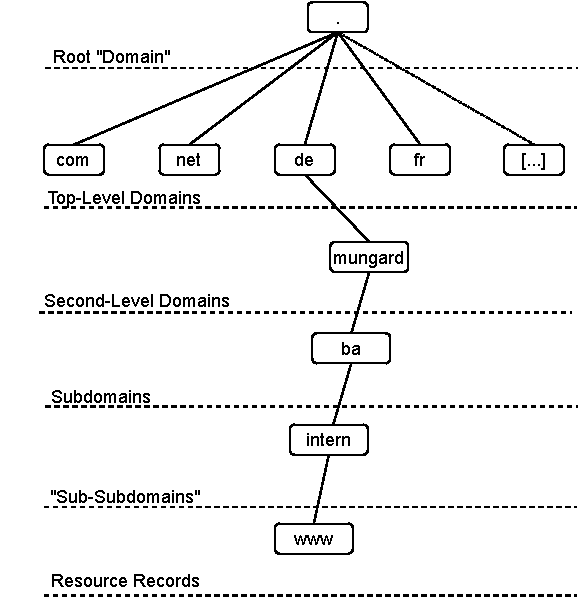
\includegraphics{Figures/dns_autoritative.pdf}
  \caption{DNS-Hierarchie}
  \label{grafik: napt}
\end{figure}\FloatBarrier

%https://www.isc.org/bind/
Soll z.B. der FQDN www.intern.ba.mungard.de. aufgelöst werden, muss der \textit{Baum} von der Wurzel \glqq .\grqq{} über die Knoten de, mungard, ... bis zum Blatt www durchlaufen werden. Man spricht von einer iterativen Auflösung. Pro Hierarchie-Ebene sind \textit{autoritative Nameserver} verantwortlich für die richtige Delegation des auflösenden Clients.\\
Das Blatt www wird auch als Resource Record bezeichnet. Für diese Arbeit sind lediglich A-Records relevant, welche FQDN nach IPv4-Adresse auflösen. Viele weitere DNS-Records existieren, z.B. für IPv6-Adressen (AAAA) oder um Mailserver (MX) für eine Domain anzugeben \cite[S.528]{Fall2011}. Ein Beispiel für einen autoritativen Nameserver ist Bind. Innerhalb des Nameservers werden Domains anhand von \textit{Zonen(-Dateien)} verwaltet

\subsection{DNS-Resolver}
Endgeräte machen diese iterative Namensauflösung typischerweise nicht selbst, sondern leiten ihre Anfragen an einen DNS-Resolver weiter (\glqq Forwarding\grqq{}). Dieser ist in folgendem Beispiel dafür verantwortlich, zu einem FQDN eine IPv4-Adresse zu finden (iterativ) und dem Endgerät zurückzuschicken.

\begin{figure}[h]
  \centering
  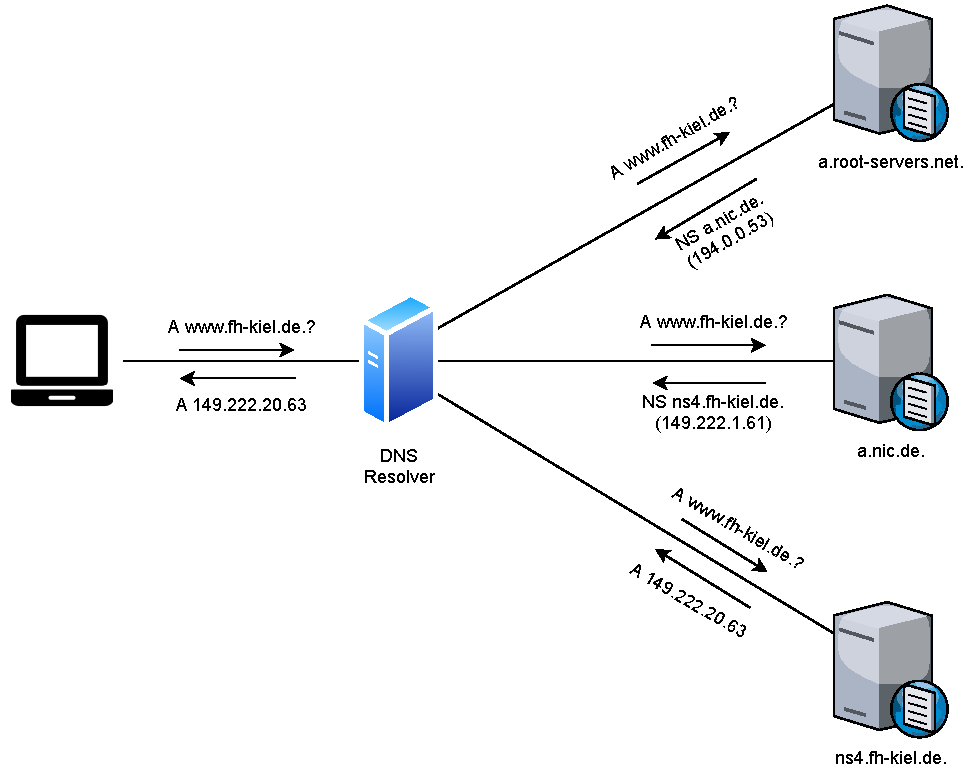
\includegraphics{Figures/dns_recursion.pdf}
  \caption{DNS-Resolver}
  \label{grafik: dns-resolver}
\end{figure}\FloatBarrier

\begin{lstlisting}[label=dig-example-fh-kiel,caption=Eine DNS-Auflösung für einen A-Record (www01.fh-kiel.de) gegen den Resolver von Google (8.8.8.8)]
$ dig www01.fh-kiel.de A @8.8.8.8

; <<>> DiG 9.11.9 <<>> www01.fh-kiel.de @8.8.8.8
;; global options: +cmd
;; Got answer:
;; ->>HEADER<<- opcode: QUERY, status: NOERROR, id: 56486
;; flags: qr rd ra ad; QUERY: 1, ANSWER: 1, AUTHORITY: 0, ADDITIONAL: 1

;; OPT PSEUDOSECTION:
; EDNS: version: 0, flags:; udp: 512
;; QUESTION SECTION:
;www01.fh-kiel.de.              IN      A

;; ANSWER SECTION:
www01.fh-kiel.de.       21425   IN      A       149.222.20.63

;; Query time: 20 msec
;; SERVER: 8.8.8.8#53(8.8.8.8)
;; WHEN: Sun May 16 15:55:30 CEST 2021
;; MSG SIZE  rcvd: 61
\end{lstlisting}



Weiterhin kann ein Resolver Einträge \textit{cachen}, um auf erneute Anfragen schneller antworten zu können.%Der letzte Punkt eines FQDN, welcher die Root-Domain repräsentiert, wird üblicherweise ausgelassen.

\subsection{Split DNS}
Split DNS ist die Möglichkeit, verschiedene Resource Records anhand der Absender-IP auszuliefern. Dafür pflegen autoritative Nameserver Access Control Lists (ACL) mit verschiedenen IP-Präfixen, um eine Fallunterscheidung treffen zu können. Dies ist z.B. relevant, wenn eine Firma zwischen internen und externen Anfragen unterscheiden muss, um den (richtigen) Zugriff auf Ressourcen zu gewährleisten.

\begin{figure}[h]
  \centering
  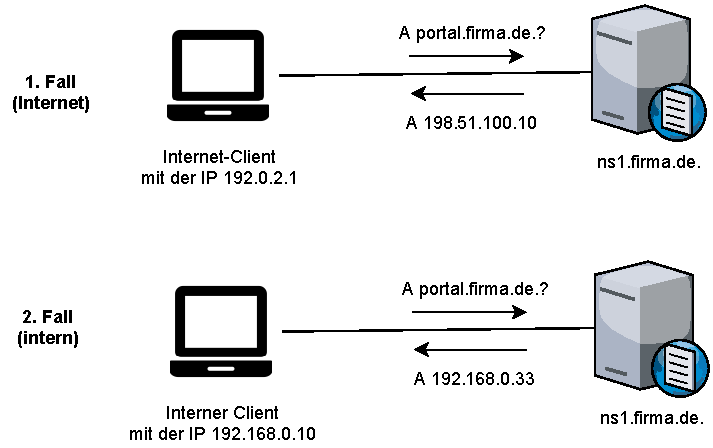
\includegraphics{Figures/dns_split_view.pdf}
  \caption{Split DNS für portal.firma.de.}
  \label{grafik: split-dns}
\end{figure}\FloatBarrier

\subsection{DNS UPDATE}
%https://datatracker.ietf.org/doc/html/rfc2136
Die Methode DNS UPDATE ist in RFC 2136 definiert und erlaubt es, autoritative Zonen eines Nameserver während der Laufzeit zu verändern. Somit müssen keine Zonen-Dateien (manuell) verändert werden. Außerdem muss der Nameserver nicht neugestartet werden, um die editierten Zonen-Dateien neu einzulesen.\\
Clients werden über eine ACL ermächtigt, diese Updates zu tätigen. Dabei kann die Absender-IP berücksichtigt werden: Allerdings ist diese Methode unsicher, da sich IPs \textit{spoofen} lassen. Sicherer ist es, mit Hilfe eines vorab ausgetauschten Schlüssels (Pre-Shared Key) eine DNS UPDATE-Nachricht zu signieren. Dies passiert mit Hilfe von Transaction Signatures (TSIG) \cite[S.911-914]{Fall2011}.
%Diese Updates werden vom Nameserver selbstständig in die Zonen-Dateien übernommen und überstehen somit einen Neustart des Servers.


\section{Virtual Private Network (VPN)}\label{vpn}
VPNs werden genutzt, um private Netzwerke über eine öffentliche Infrastruktur abbilden zu können. Dies erfolgt zwischen VPN-Endpunkten über eine gängige Enkapsulierung, z.B. Generic Routing Encapsulation (GRE), Encapsulating Security Payload (ESP) oder OpenVPN.

In diesem Beispiel werden Daten von Client A zu Client B über das Internet zwischen Router R1 und Router R2 enkapsuliert. R2 empfängt das Datenpaket, packt es aus und sendet es in der ursprünglichen Form weiter an Client B. Das Diagramm ist nicht spezifisch für eine bestimmte VPN-Technologie, sondern soll die grundsätzliche Idee verdeutlichen. Weiterhin können, je nach Technologie, Nutzdaten verschlüsselt werden. 

\begin{figure}[h]
  \centering
  \includegraphics{Figures/}
  \caption{Übertragung eines IP-Pakets über einen VPN-Tunnel}
  \label{grafik: vpn-example}
\end{figure}\FloatBarrier

%Quelle
Die in dieser Arbeit verwendeten VPN-Technologien sind IPSEC und OpenVPN. IPSEC wird u.a. für die Vernetzung von Standorten, auch Site-to-Site (S2S) genannt, genutzt und arbeitet auf OSI-Schicht 3. Ebenso dient es zur \glqq Einwahl\grqq{} in (Firmen-)Netzwerken.  IPSEC wird meist im Geschäftsumfeld genutzt und es exisitieren viele herstellerabhängige Implementationen.\\
OpenVPN ist ein Open Source-Projekt, es nutzt Transport Layer Security (TLS) für die verschlüsselte Übertragung von Daten via UDP. Das Protokoll ist auf OSI-Schicht 7 zu finden. Es wird vor allem für Client-to-Site-Verbindungen genutzt (C2S): Passende Software ist für viele verschiedene Plattformen verfügbar (Windows, Linux, Mac, Android,...) und sowohl Client als auch Server-Applikation sind kostenfrei erhältlich.

%ROUTE BASED VS POLICY BASED?
Angesprochene MTU-Probleme / MSS (s.o.)